\documentclass[10pt, aspectratio=169]{beamer}

\usetheme{Madrid}
\usecolortheme{seahorse}
\setbeamertemplate{navigation symbols}{}
\setbeamertemplate{footline}[frame number]
\definecolor{metallicgold}{HTML}{D4AF37}

\usepackage{amsmath, amssymb, booktabs, graphicx, multicol, subcaption}
\graphicspath{{./}{../}}
\usepackage[T1]{fontenc}
\usepackage{lmodern}
\usepackage{tikz}

\definecolor{myblue}{RGB}{0,73,135}
\definecolor{myred}{RGB}{180,30,30}
\definecolor{mygreen}{RGB}{0,120,60}
\setbeamercolor{title}{fg=myred}
\setbeamercolor{frametitle}{fg=myred}
\setbeamercolor{block title}{bg=metallicgold,fg=black}
\setbeamercolor{item}{fg=myred}
\setbeamercolor{caption name}{fg=myred}

\title[Replication: Natural Disasters \& Growth]{Replication Study:\\
\textit{The Growth Aftermath of Natural Disasters}}
\subtitle{Fomby, Ikeda \& Loayza (2013) --- Journal of Applied Econometrics}
\author{Toprak Özdemir}
\institute{EC 532 - Bogazici University}
\date{May 2026}

\begin{document}

\begin{frame}
\titlepage
\end{frame}

\begin{frame}{Outline}
\tableofcontents
\end{frame}

\section{What Does the Paper Aim to Achieve?}

\begin{frame}{Research Question}
\begin{block}{Core Question}
\textbf{What happens to a country's economic growth after a natural disaster?}
\end{block}
\vspace{0.5em}
The paper goes beyond simple averages and asks:
\begin{itemize}
    \item How does GDP growth respond \textbf{dynamically} over the years following four types of disasters: \textit{droughts, floods, earthquakes, and storms}?
    \item Do the effects differ across \textbf{sectors} (agriculture vs.\ non-agriculture)?
    \item Do \textbf{developing} vs.\ \textbf{developed} countries respond differently?
    \item Do \textbf{severe} disasters have qualitatively different effects than moderate ones?
\end{itemize}
\end{frame}

\begin{frame}{Why This Paper Matters}
\begin{columns}
\begin{column}{0.55\textwidth}
\textbf{Key contributions:}
\begin{enumerate}
    \item Applies a \textbf{Panel VARX} model to capture dynamic, multi-variable interactions
    \item Introduces a \textbf{Bootstrap Bias Correction} (BSBC) to fix the well-known Nickell bias in dynamic panels
    \item Provides a \textbf{nuanced view}: not all disasters are bad, and not all sectors are affected equally
\end{enumerate}
\end{column}
\begin{column}{0.42\textwidth}
\textbf{Data at a glance:}
\begin{itemize}
    \item 84 countries (60 developing, 24 developed)
    \item 48 years (1960--2007)
    \item Unbalanced panel
    \item 6 endogenous + 6 exogenous variables per model
\end{itemize}
\end{column}
\end{columns}
\end{frame}

\section{Data \& Methodology}

\begin{frame}{The Model: Panel VARX(2,2)}
The core econometric model is a \textbf{fixed-effects} Panel VARX:
\[
y_{i,t} = \alpha_i + \Phi_1 y_{i,t-1} + \Phi_2 y_{i,t-2} + \Theta_0 x_{i,t} + \Theta_1 x_{i,t-1} + \Theta_2 x_{i,t-2} + \varepsilon_{i,t}
\]

\begin{columns}
\hspace{5mm}
\begin{column}{0.48\textwidth}
\textbf{Endogenous} ($y_{i,t}$, $K=6$):
\begin{itemize}
    \item GDP (or sectoral) growth
    \item Capital formation growth
    \item CPI inflation
    \item Trade openness growth
    \item Gov.\ consumption growth
    \item Financial depth growth
\end{itemize}
\end{column}
\begin{column}{0.48\textwidth}
\textbf{Exogenous} ($x_{i,t}$, $dis=6$):
\begin{itemize}
    \item Drought intensity
    \item Flood intensity
    \item Earthquake intensity
    \item Storm intensity
    \item Terms of trade growth
    \item World GDP growth
\end{itemize}
\end{column}
\end{columns}
\end{frame}

\begin{frame}{Descriptive Statistics (from preprocessed data)}
\begin{table}[h]
\centering
\vspace{-0.3em}
\resizebox{0.95\textwidth}{!}{
\begin{tabular}{l rrrr rrrr}
\toprule
& \multicolumn{4}{c}{\textbf{Developing} ($N = 60$)} & \multicolumn{4}{c}{\textbf{Developed} ($N = 24$)} \\
\cmidrule(lr){2-5} \cmidrule(lr){6-9}
\textbf{Variable} & \textbf{Mean} & \textbf{Std} & \textbf{Min} & \textbf{Max} & \textbf{Mean} & \textbf{Std} & \textbf{Min} & \textbf{Max} \\
\midrule
GDP growth           & 0.016 & 0.051 & $-$0.438 & 0.377 & 0.021 & 0.023 & $-$0.128 & 0.111 \\
Capital formation gr & 0.006 & 0.157 & $-$1.492 & 1.586 & $-$0.004 & 0.058 & $-$0.264 & 0.239 \\
Inflation rate       & 0.128 & 0.190 & $-$0.124 & 2.626 & 0.059 & 0.053 & $-$0.101 & 0.356 \\
Trade openness gr    & 0.013 & 0.115 & $-$0.773 & 0.667 & 0.015 & 0.065 & $-$0.302 & 0.328 \\
Gov.\ consumption gr & 0.000 & 0.111 & $-$0.753 & 0.993 & 0.007 & 0.036 & $-$0.135 & 0.208 \\
Financial depth gr   & 0.016 & 0.163 & $-$1.853 & 1.042 & 0.029 & 0.122 & $-$1.005 & 1.356 \\
\midrule
Drought intensity    & 0.079 & 0.285 & 0.000 & 2.000 & 0.009 & 0.095 & 0.000 & 1.000 \\
Flood intensity      & 0.300 & 0.589 & 0.000 & 5.000 & 0.066 & 0.282 & 0.000 & 2.000 \\
Earthquake intensity & 0.047 & 0.226 & 0.000 & 2.000 & 0.021 & 0.159 & 0.000 & 2.000 \\
Storm intensity      & 0.139 & 0.545 & 0.000 & 7.000 & 0.061 & 0.264 & 0.000 & 3.000 \\
\midrule
TOT growth           & $-$0.003 & 0.122 & $-$0.709 & 0.706 & $-$0.001 & 0.042 & $-$0.226 & 0.241 \\
World GDP growth     & 0.017 & 0.012 & $-$0.012 & 0.043 & 0.016 & 0.012 & $-$0.012 & 0.043 \\
\bottomrule
\end{tabular}
}
\vspace{0.2em} \\
\footnotesize{Developing countries face far more frequent and intense disasters, with higher growth volatility.}
\end{table}
\end{frame}

\begin{frame}{Measuring Disaster Intensity}
\textbf{Step 1: Event-level indicator} (from EM-DAT database)

For each event $j$ of disaster type $k$ in country $i$, year $t$:
\[
\text{intensity}^k_{i,t,j} =
\begin{cases}
1 & \text{if } \dfrac{\text{fatalities}^k_{i,t,j} + 0.3 \times \text{total\_affected}^k_{i,t,j}}{\text{population}_{i,t}} > \underbrace{0.0001}_{\text{0.01\%}} \\[6pt]
0 & \text{otherwise}
\end{cases}
\]

\textbf{Step 2: Country-year aggregate}
\[
ND_{i,t}(k) = \sum_{j=1}^{J} \text{intensity}^k_{i,t,j}
\]
This counts how many type-$k$ events exceeded the threshold in a given country-year.

\vspace{0.3em}
\textbf{Severe disasters}: Threshold is 100 times higher ($> 0.01$, i.e.\ 1\% of population). Severe disaster dummies are added as \textbf{extra} regressors in the severe model ($dis = 10$ instead of 6).
\end{frame}

\begin{frame}{Lag Order Selection: Information Criteria}
I replicated the information criteria computation for all three lag orders:

\vspace{0.3em}
\begin{table}[h]
\centering
\begin{tabular}{c cc l}
\toprule
\textbf{Lag order ($p = q$)} & \textbf{AIC} & \textbf{SBC} & \textbf{Selected by} \\
\midrule
$p = q = 1$ & $-10.169$ & $\mathbf{-9.849}$ & $\leftarrow$ SBC (most conservative) \\
$p = q = 2$ & $-10.223$ & $-9.690$ & $\leftarrow$ \textbf{Paper's choice} \\
$p = q = 3$ & $\mathbf{-10.252}$ & $-9.505$ & $\leftarrow$ AIC (most parameters) \\
\bottomrule
\end{tabular}
\vspace{0.3em}
\end{table}

\vspace{0.2em}
\begin{itemize}
    \item \textbf{AIC} favors $p = q = 3$ (lower is better, but AIC tends to overfit)
    \item \textbf{SBC} favors $p = q = 1$ (penalizes complexity more heavily)
    \item Authors chose $p = q = 2$ as a \textbf{compromise}, balancing fit and parsimony
\end{itemize}
\end{frame}

\begin{frame}{Estimation: The LSDV and Its Problem}
\textbf{Step 1: Stacking and The Within Transformation (LSDV)}

To estimate the system, we stack observations over time and across countries. Let $y$ be the stacked $T \times 6$ matrix of dependent variables, and $Z$ be the stacked matrix of all right-hand side variables (lagged $y$ and exogenous $x$).
\\

To remove the country fixed effects $\alpha_i$, the data is pre-multiplied by the \textbf{annihilator matrix}:
\[
A_i = I_{T_i} - \frac{1}{T_i} \iota_{T_i} \iota_{T_i}'
\]
This subtracts the country-level time mean from all variables, eliminating $\alpha_i$. Then, the LSDV estimator is:
\[
\hat{\delta} = (Z'AZ)^{-1}Z'Ay
\]

\begin{alertblock}{The Nickell Bias Problem}
In a dynamic panel (with lagged $y_{i,t-1}$), the within transformation creates a \textbf{mechanical correlation} between the transformed regressor $(y_{i,t-1} - \bar{y}_i)$ and the transformed error $(\varepsilon_{i,t} - \bar{\varepsilon}_i)$. This makes the LSDV estimator \textbf{inconsistent} for moderate $T$ (here $T \approx 35$).
\end{alertblock}
\end{frame}

\begin{frame}{From LSDV to Mean Responses}
    The LSDV estimator $\hat{\delta}$ gives us the \textbf{short-run coefficients}: the autoregressive matrices ($\hat{\Phi}_1, \hat{\Phi}_2$) and the exogenous impact matrices ($\hat{\Theta}_0, \hat{\Theta}_1, \hat{\Theta}_2$).
    
    \vspace{0.3em}
    \textbf{Inverting the VARX System:}
    \begin{itemize}
        \item To find the dynamic path of the economy after a disaster, we invert the VARX into its multiplier form: $y_{i,t} = \hat{\Psi}(L)x_{i,t} + \text{error}$
        \item The lag polynomial $\hat{\Psi}(L) = \hat{\Phi}(L)^{-1}\hat{\Theta}(L)$ contains the mean responses ($\hat{\Psi}_s$).
    \end{itemize}

    \vspace{0.3em}
    \textbf{Recursive Calculation of Mean Responses ($\hat{\Psi}_s$):}
    Instead of complex matrix inversion, our code calculates the responses recursively:
    \begin{align*}
        \textbf{Year 0 (Immediate):} \quad & \hat{\Psi}_0 = \hat{\Theta}_0 \\
        \textbf{Year 1 (Delay 1):} \quad & \hat{\Psi}_1 = \hat{\Phi}_1\hat{\Psi}_0 + \hat{\Theta}_1 \\
        \textbf{Year 2 (Delay 2):} \quad & \hat{\Psi}_2 = \hat{\Phi}_1\hat{\Psi}_1 + \hat{\Phi}_2\hat{\Psi}_0 + \hat{\Theta}_2 \\
        \textbf{Year 3+ (Delay s > 2):} \quad & \hat{\Psi}_s = \hat{\Phi}_1\hat{\Psi}_{s-1} + \hat{\Phi}_2\hat{\Psi}_{s-2}
    \end{align*}
    
    \footnotesize \textit{Note: This recursive logic is mathematically exactly what the Nickell Bias distorts, which is why the authors apply the bootstrap correction directly to these $\hat{\Psi}_s$ matrices.}
\end{frame}

\begin{frame}{BSBC Algorithm -- Step by Step (from the code)}
\textbf{Phase 1: Initial estimation \& residual preparation}
\begin{enumerate}
    \item Compute LSDV estimate: $\hat{\delta} = (Z'AZ)^{-1}Z'Ay$
    \item Extract fixed effects: $\hat{\alpha}_i = \frac{1}{T_i}(y - Z\hat{\delta}')' D e_i$
    \begin{itemize}
        \item \footnotesize \textit{Where $D$ is a $T \times N$ matrix of country dummy variables, and $e_i$ is an $N \times 1$ selection vector with a $1$ in the $i$-th position and $0$ elsewhere.} \normalsize
    \end{itemize}
    \item Compute raw residuals: $\hat{\varepsilon} = y - D\hat{\alpha}' - Z\hat{\delta}'$
    \item \textbf{Rescale} residuals using the projection matrix diagonal:
    \[
    \hat{\varepsilon}^r_{i,t} = \sqrt{\frac{T_i}{T_i - 1}} \left( \frac{\hat{\varepsilon}_{i,t}}{\sqrt{m_{i,t}}} - \frac{1}{T_i}\sum_{k=1}^{T_i}\frac{\hat{\varepsilon}_{i,k}}{\sqrt{m_{i,k}}} \right)
    \]
    where $m_{i,t}$ is the diagonal of $M = A - AZ(Z'AZ)^{-1}Z'A$.
\end{enumerate}

\vspace{0.3em}
The rescaling corrects for \textbf{degrees of freedom} and ensures the bootstrapped residuals have the right variance structure.
\end{frame}

\begin{frame}{BSBC Algorithm -- The Bootstrap Loop}
\textbf{Phase 2: Bootstrap resampling ($B = 1000$ times)}

For each $j = 1, \ldots, B$:
\begin{enumerate}
    \item Draw $T$ integers at random $\rightarrow$ resample residuals $\hat{\varepsilon}^{b(j)}$
    \item \textbf{Recursively} generate synthetic data:
    \[
    y^{b(j)} = D\hat{\alpha}' + Z^{b(j)}\hat{\delta} + \hat{\varepsilon}^{b(j)}
    \]
    \vspace{-5mm}
    \begin{itemize}
        \item \footnotesize \textit{Where $Z^{b(j)}$ updates the lagged endogenous variables with the newly generated $y$ data, but keeps the exogenous disaster shocks $x$ fixed.} \normalsize
    \end{itemize}
    \item Re-estimate LSDV on synthetic data: $\hat{\delta}^{b(j)} = (Z^{b(j)\prime}AZ^{b(j)})^{-1}Z^{b(j)\prime}Ay^{b(j)}$
\end{enumerate}
\end{frame}

\begin{frame}{BSBC Algorithm -- Correcting the Bias}
    \textbf{Phase 3: Bias Correction}
    
    \vspace{0.3em}
    \begin{enumerate}
        \item \textbf{The Problem:} Our standard LSDV estimate ($\hat{\Psi}_s$) contains Nickell Bias.
        \item \textbf{The Simulation:} We create $B=1000$ synthetic "fake economies" where our biased estimate ($\hat{\Psi}_s$) is treated as the absolute, known truth.
        \item \textbf{Measuring the Bias:} We re-estimate the LSDV model on these synthetic economies to get $\hat{\Psi}_s^{b(j)}$. The average of these fake estimates minus the "truth" of the fake economy gives us the exact simulated bias:
        \[ \text{Simulated Bias} = \left( \frac{1}{B}\sum_{j=1}^{B}\hat{\Psi}_s^{b(j)} \right) - \hat{\Psi}_s \]
        \item \textbf{The Correction:} We subtract this simulated bias from our original estimate:
        \[ \tilde{\Psi}_s = \hat{\Psi}_s - \text{Simulated Bias} \]
        \[ \tilde{\Psi}_s = \hat{\Psi}_s - \left( \frac{1}{B}\sum_{j=1}^{B}\hat{\Psi}_s^{b(j)} - \hat{\Psi}_s \right) \implies \boxed{\tilde{\Psi}_s = 2\hat{\Psi}_s - \frac{1}{B}\sum_{j=1}^{B}\hat{\Psi}_s^{b(j)}} \]
    \end{enumerate}
\end{frame}

\begin{frame}{Statistical Inference: Nested Bootstrap}
To build \textbf{confidence intervals} for the bias-corrected estimates, the script runs a \textbf{nested bootstrap}: for each of the $B = 1000$ outer samples, it runs \textbf{another} full BSBC procedure ($B = 1000$ inner).

\vspace{0.3em}
\begin{center}
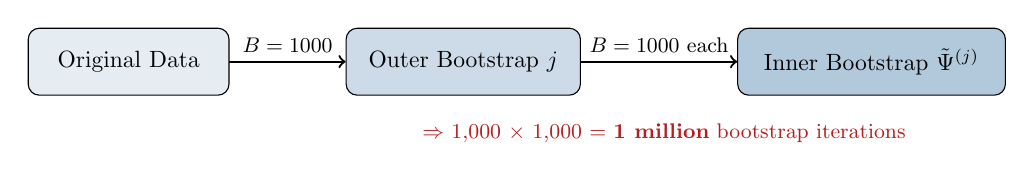
\begin{tikzpicture}[scale=0.85, every node/.style={scale=0.85}]
    \node[draw, rounded corners, fill=myblue!10, minimum width=3cm, minimum height=1cm] (data) at (0,0) {Original Data};
    \node[draw, rounded corners, fill=myblue!20, minimum width=3.5cm, minimum height=1cm] (outer) at (5,0) {Outer Bootstrap $j$};
    \node[draw, rounded corners, fill=myblue!30, minimum width=4cm, minimum height=1cm] (inner) at (11.1,0) {Inner Bootstrap $\tilde{\Psi}^{(j)}$};
    \draw[->, thick] (data) -- node[above, font=\small]{$B=1000$} (outer);
    \draw[->, thick] (outer) -- node[above, font=\small]{$B=1000$ each} (inner);
    \node[below=0.3cm, font=\small\color{myred}] at (8,-0.5) {$\Rightarrow$ 1,000 $\times$ 1,000 = \textbf{1 million} bootstrap iterations};
\end{tikzpicture}
\end{center}

\vspace{0.3em}
The sorted $\{\tilde{\Psi}^{(1)}, \ldots, \tilde{\Psi}^{(B)}\}$ gives the 5th/10th/90th/95th percentiles for confidence intervals. \\[0.5em]
\textbf{LSDV robustness check}: Uses 30,000 Monte Carlo draws from a multivariate normal distribution, which is much cheaper (computationally) but relies on asymptotic normality.
\end{frame}

\section{Replication: My Estimations and Findings}

\begin{frame}{Replication Strategy}
\textbf{Original}: MATLAB estimation scripts + Stata data preparation + pre-processed CSV/XLS datasets in the replication package.

\vspace{0.3em}
\textbf{Our approach}: I used the \textbf{pre-processed datasets} directly from the replication package and translated the \textbf{MATLAB estimation code} to Python.
\begin{itemize}
    \item \texttt{apply\_LSDV.py} $\rightarrow$ LSDV estimator with Monte Carlo inference
    \item \texttt{apply\_BSBC.py} $\rightarrow$ Bootstrap bias-corrected estimator (main results)
    \item \texttt{apply\_severe\_LSDV.py} $\rightarrow$ Severe disaster model (LSDV)
    \item \texttt{apply\_severe\_BSBC.py} $\rightarrow$ Severe disaster model (BSBC)
    \item \texttt{helpers.py} / \texttt{helpers\_numba.py} $\rightarrow$ Shared functions (\texttt{psimat}, \texttt{meanpsi}, \texttt{btst})
\end{itemize}
\vspace{0.3em}
Key libraries: \texttt{numpy}, \texttt{pandas}, \texttt{matplotlib}, \texttt{numba}
\end{frame}

\begin{frame}{Replication vs. Original Results: All Growth Responses}
    \begin{table}
        \centering
        \vspace{-4mm}
        \caption{\footnotesize Mean responses of GDP growth to natural disaster shocks (BSBC, developing countries)}
        \renewcommand{\arraystretch}{0.97} 
        \vspace{-2mm}
        \resizebox{0.8\textwidth}{!}{
        \begin{tabular}{llcccccc}
            \midrule
            & & \multicolumn{2}{c}{GDP growth} & \multicolumn{2}{c}{Agr. growth} & \multicolumn{2}{c}{Non-agr. growth} \\
            \cmidrule(lr){3-4} \cmidrule(lr){5-6} \cmidrule(lr){7-8}
            Disaster & Period & Orig. & Rep. & Orig. & Rep. & Orig. & Rep. \\
            \midrule
            Droughts    & Year 0            & $-0.0160^{**}$ & $-0.0157^{**}$ & $-0.0349^{**}$ & $-0.0353^{**}$ & $-0.0076^{**}$ & $-0.0076^{**}$ \\
                        & Year 1            & $-0.0009$      & $-0.0006$      & $0.0214^{**}$  & $0.0214^{**}$  & $-0.0043$      & $-0.0045$ \\
                        & Year 2            & $-0.0034$      & $-0.0037$      & $-0.0050$      & $-0.0055$      & $-0.0055^{*}$  & $-0.0055^{*}$ \\
                        & Cumulative        & $-0.0214^{**}$ & $-0.0212^{**}$ & $-0.0192^{**}$ & $-0.0200^{**}$ & $-0.0198^{**}$ & $-0.0200^{**}$ \\
            [0.5ex]
            Floods      & Year 0            & $0.0017$       & $0.0015$       & $0.0033$       & $0.0036$       & $0.0008$       & $0.0009$ \\
                        & Year 1            & $0.0012$       & $0.0012$       & $0.0064^{*}$   & $0.0061^{*}$   & $0.0001$       & $0.0002$ \\
                        & Year 2            & $0.0029^{*}$   & $0.0031$       & $-0.0002$      & $0.0002$       & $0.0040^{*}$   & $0.0040^{**}$ \\
                        & Cumulative        & $0.0062^{*}$   & $0.0061^{*}$   & $0.0090^{**}$  & $0.0092^{**}$  & $0.0061^{*}$   & $0.0062^{*}$ \\
            [0.5ex]
            Earthquakes & Year 0            & $0.0046$       & $0.0049$       & $-0.0008$      & $-0.0009$      & $0.0046$       & $0.0044$ \\
                        & Year 1            & $0.0049$       & $0.0049$       & $-0.0020$      & $-0.0017$      & $0.0071^{*}$   & $0.0071^{*}$ \\
                        & Year 2            & $-0.0038$      & $-0.0038$      & $-0.0072$      & $-0.0076$      & $-0.0054$      & $-0.0055$ \\
                        & Cumulative        & $0.0067$       & $0.0070$       & $-0.0074$      & $-0.0075$      & $0.0054$       & $0.0051$ \\
            [0.5ex]
            Storms      & Year 0            & $-0.0028$      & $-0.0028$      & $0.0021$       & $0.0020$       & $-0.0038$      & $-0.0038$ \\
                        & Year 1            & $-0.0009$      & $-0.0009$      & $-0.0048$      & $-0.0049$      & $0.0021$       & $0.0021$ \\
                        & Year 2            & $0.0011$       & $0.0010$       & $0.0062$       & $0.0062$       & $0.0004$       & $0.0004$ \\
                        & Cumulative        & $-0.0020$      & $-0.0021$      & $0.0026$       & $0.0025$       & $-0.0005$      & $-0.0005$ \\
            \midrule
                        & Countries         & 60         & 60         & 60         & 60         & 60         & 60 \\
                        & Sample period     & '60--'07   & '60--'07   & '60--'07   & '60--'07   & '60--'07   & '60--'07 \\
                        & Observations      & 2097       & 1866       & 1878       & 1644       & 1863       & 1635 \\
            \bottomrule
            \multicolumn{8}{l}{\scriptsize \textit{Note:} $^{*}$ significant at one-tail 10\% level, $^{**}$ at 5\% level.}
        \end{tabular}
        }
    \end{table}
\end{frame}

\begin{frame}{Replication vs. Original Results: GDP Growth (Developed)}
    \begin{table}
        \centering
        \vspace{-4mm}
        \caption{\footnotesize Mean responses of GDP growth to natural disaster shocks (BSBC, developed countries)}
        \vspace{-2mm}
        \resizebox{0.45\textwidth}{!}{
        \begin{tabular}{llcc}
            \midrule
            & & Original Paper & Replicated \\
            Disaster & Period & GDP growth & GDP growth \\
            \midrule
            Droughts    & Year 0            & $0.0102$  & $0.0105$ \\
                        & Year 1            & $-0.0028$ & $-0.0026$ \\
                        & Year 2            & $0.0034$  & $0.0035$ \\
                        & Year 3            & $0.0022$  & $0.0024$ \\
                        & Cumulative effect & $0.0129$  & $0.0138$ \\
            [0.5ex]
            Floods      & Year 0            & $0.0018$  & $0.0018$ \\
                        & Year 1            & $0.0015$  & $0.0016$ \\
                        & Year 2            & $0.0024$  & $0.0026$ \\
                        & Year 3            & $0.0012$  & $0.0013$ \\
                        & Cumulative effect & $0.0069$  & $0.0073$ \\
            [0.5ex]
            Earthquakes & Year 0            & $0.0003$  & $-0.0002$ \\
                        & Year 1            & $-0.0044$ & $-0.0047$ \\
                        & Year 2            & $0.0030$  & $0.0025$ \\
                        & Year 3            & $0.0024$  & $0.0023$ \\
                        & Cumulative effect & $0.0013$  & $-0.0001$ \\
            [0.5ex]
            Storms      & Year 0            & $0.0000$  & $-0.0000$ \\
                        & Year 1            & $-0.0002$ & $-0.0001$ \\
                        & Year 2            & $0.0014$  & $0.0014$ \\
                        & Year 3            & $-0.0004$ & $-0.0004$ \\
                        & Cumulative effect & $0.0008$  & $0.0008$ \\
            \midrule
                        & Number of countries    & 24         & 24 \\
                        & Sample period          & 1960--2007 & 1960--2007 \\
                        & Number of observations & 853        & 775 \\
            \bottomrule
            \multicolumn{4}{l}{\scriptsize \textit{Note:} $^{*}$ significant at one-tail 10\% level, $^{**}$ at 5\% level.}
        \end{tabular} }
    \end{table}
\end{frame}
\begin{frame}{Replicated Results: LSDV Robustness Check}

\begin{table}[h]
\centering
\caption{\small Mean responses of GDP growth (developing countries)}
\vspace{-0.3em}
\resizebox{0.75\textwidth}{!}{
\begin{tabular}{ll cc}
\toprule
\textbf{Disaster} & \textbf{Period} & \textbf{LSDV} & \textbf{BSBC} \\
\midrule
Droughts & Year 0 & $-0.0157^{**}$ & $-0.0157^{**}$ \\
         & Cumulative effect & $-0.0208^{**}$ & $-0.0212^{**}$ \\
\midrule
Floods   & Year 2 & $\phantom{-}0.0029^{*}$ & $\phantom{-}0.0029^{*}$ \\
         & Cumulative effect & $\phantom{-}0.0059^{*}$ & $\phantom{-}0.0062^{*}$ \\
\midrule
Earthquakes & Cumulative effect & $\phantom{-}0.0071$ & $\phantom{-}0.0067$ \\
\midrule
Storms   & Cumulative effect & $-0.0021$ & $\phantom{-}0.0020$ \\
\bottomrule
\end{tabular}
}
\vspace{0.2em} \\
\footnotesize{LSDV results are consistent with BSBC in direction and significance,\\confirming the robustness of the findings even without bias correction.}
\end{table}
\end{frame}

\begin{frame}{Mean Response Figures: Drought Shock (BSBC, developing countries)}
    \begin{figure}[H]
    \centering
    \begin{subfigure}[b]{0.32\textwidth}
        \centering
        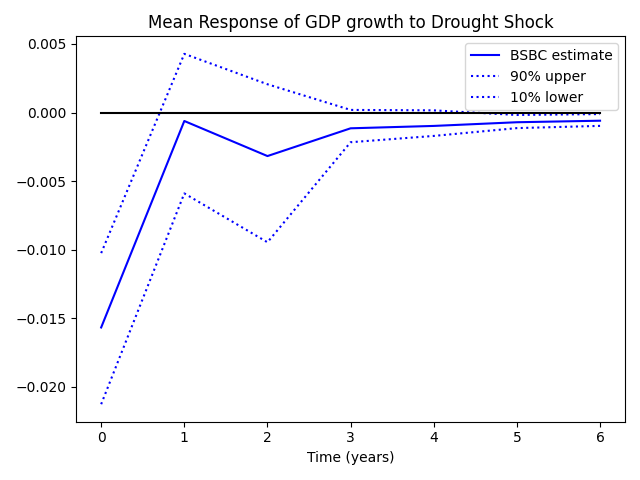
\includegraphics[width=\textwidth]{figures/BSBC/Developing/moderate/BSBC_devgrow_drought.png} 
    \end{subfigure}
    \begin{subfigure}[b]{0.32\textwidth}
        \centering
        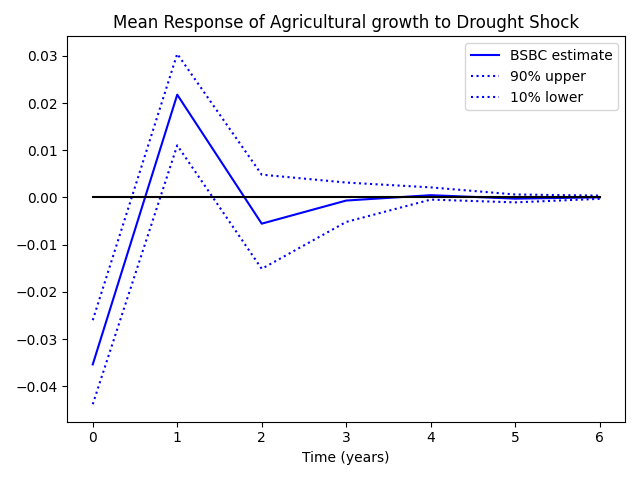
\includegraphics[width=\textwidth]{figures/BSBC/Developing/moderate/BSBC_devagr_drought.png}
    \end{subfigure}
    \begin{subfigure}[b]{0.32\textwidth}
        \centering
        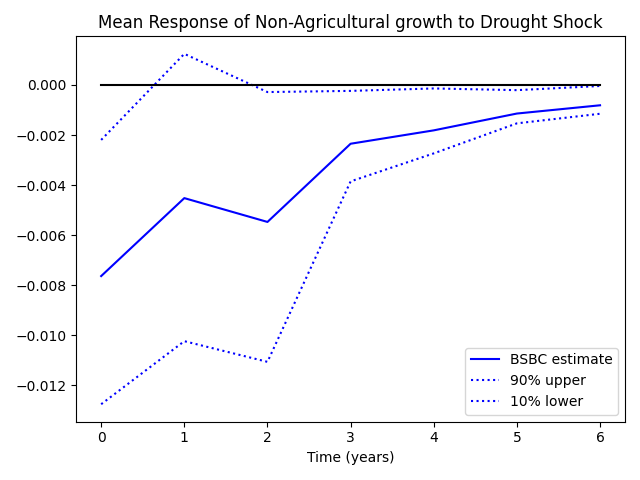
\includegraphics[width=\textwidth]{figures/BSBC/Developing/moderate/BSBC_devnon_drought.png}
    \end{subfigure}
    \caption{Replicated BSBC mean responses to a drought shock (GDP, agricultural, and non-agricultural growth). Compare with Figure 1 of Fomby, Ikeda, and Loayza (2013, p.~426).}
    \label{fig:drought_bsbc}
\end{figure}
\end{frame}

\begin{frame}{Mean Response Figures: Flood Shock (BSBC, developing countries)}
    \begin{figure}[H]
    \centering
    \begin{subfigure}[b]{0.32\textwidth}
        \centering
        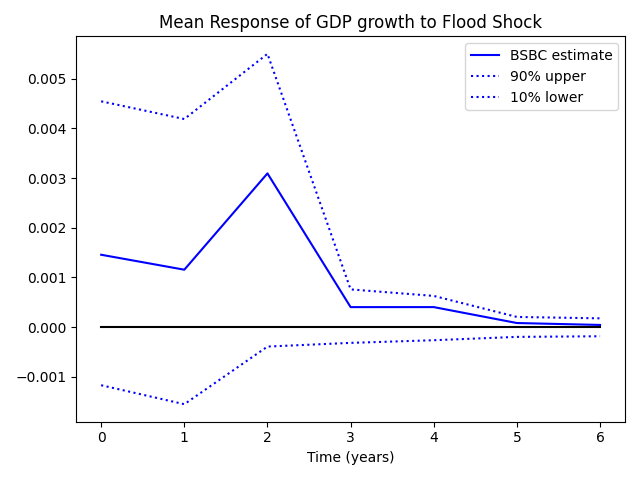
\includegraphics[width=\textwidth]{figures/BSBC/Developing/moderate/BSBC_devgrow_flood.png} 
    \end{subfigure}
    \begin{subfigure}[b]{0.32\textwidth}
        \centering
        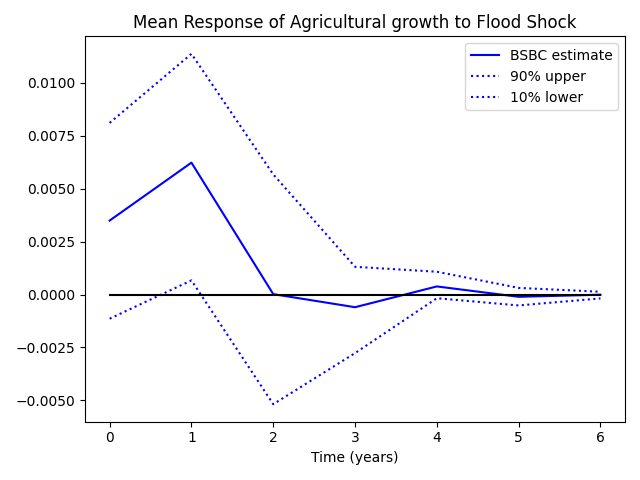
\includegraphics[width=\textwidth]{figures/BSBC/Developing/moderate/BSBC_devagr_flood.png}
    \end{subfigure}
    \begin{subfigure}[b]{0.32\textwidth}
        \centering
        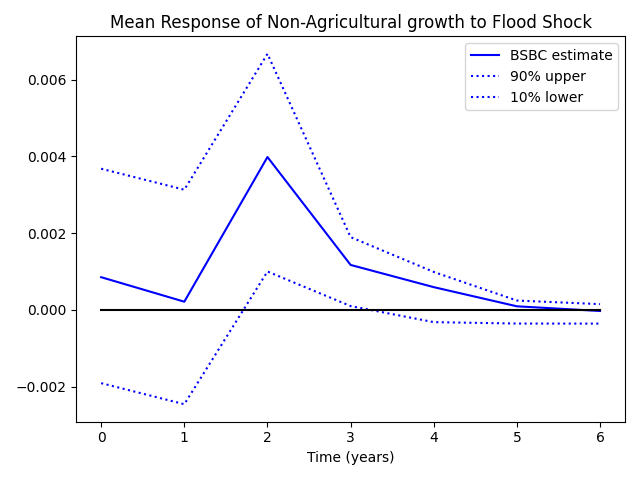
\includegraphics[width=\textwidth]{figures/BSBC/Developing/moderate/BSBC_devnon_flood.png}
    \end{subfigure}
    \caption{Replicated BSBC mean responses to a flood shock (GDP, agricultural, and non-agricultural growth). Compare with Figure 2 of Fomby, Ikeda, and Loayza (2013, p.~427).}
    \label{fig:flood_bsbc}
\end{figure}
\end{frame}

\begin{frame}{Mean Response Figures: Flood Shock (LSDV, developing countries)}
    \begin{figure}[H]
    \centering
    \begin{subfigure}[b]{0.32\textwidth}
        \centering
        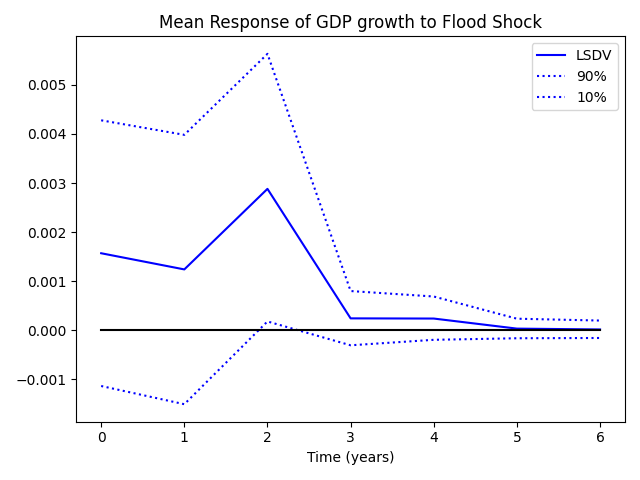
\includegraphics[width=\textwidth]{figures/LSDV/Developing/moderate/LSDV_devgrow_flood.png} 
    \end{subfigure}
    \begin{subfigure}[b]{0.32\textwidth}
        \centering
        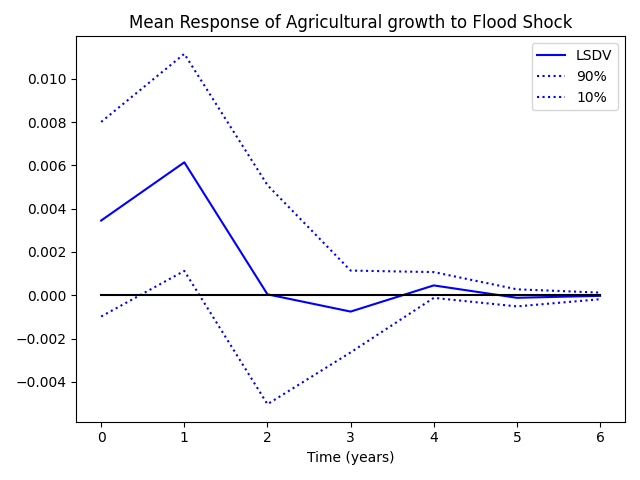
\includegraphics[width=\textwidth]{figures/LSDV/Developing/moderate/LSDV_devagr_flood.png}
    \end{subfigure}
    \begin{subfigure}[b]{0.32\textwidth}
        \centering
        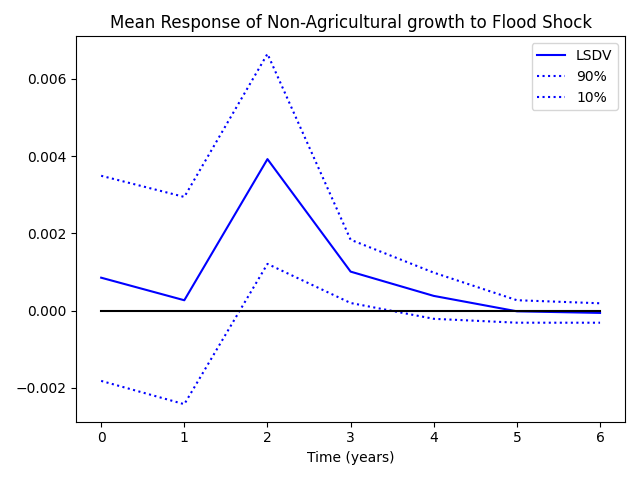
\includegraphics[width=\textwidth]{figures/LSDV/Developing/moderate/LSDV_devnon_flood.png}
    \end{subfigure}
    \caption{LSDV figures are consistent with BSBC, which shows the robustness of findings.}
    \label{fig:guidance_scale}
\end{figure}
\end{frame}

\begin{frame}{Replication vs. Original: Moderate vs. Severe (GDP Growth)}
    \begin{table}
        \centering
        \renewcommand{\arraystretch}{0.95} 
        \resizebox{0.6\textwidth}{!}{
        \begin{tabular}{llcccc}
            \toprule
            \multicolumn{6}{l}{Table: Mean responses of GDP growth to moderate/severe disaster shocks (BSBC, developing)} \\
            \midrule
            & & \multicolumn{2}{c}{Moderate Disasters} & \multicolumn{2}{c}{Severe Disasters} \\
            \cmidrule(lr){3-4} \cmidrule(lr){5-6}
            Disaster & Period & Orig. & Rep. & Orig. & Rep. \\
            \midrule
            Droughts    & Year 0            & $-0.0092^{*}$  & $-0.0093^{*}$  & $-0.0225^{**}$ & $-0.0223^{**}$ \\
                        & Year 1            & $-0.0086^{*}$  & $-0.0083^{*}$  & $0.0054$       & $0.0054$ \\
                        & Year 2            & $-0.0070$      & $-0.0065^{*}$  & $0.0001$       & $0.0005$ \\
                        & Year 3            & $-0.0019$      & $-0.0019$      & $-0.0007$      & $-0.0006$ \\
                        & Cumulative effect & $-0.0266^{**}$ & $-0.0261^{**}$ & $-0.0177^{*}$  & $-0.0170^{**}$ \\
            [0.5ex]
            Floods      & Year 0            & $0.0013$       & $0.0013$       & $-0.0011$      & $-0.0010$ \\
                        & Year 1            & $0.0017$       & $0.0017$       & $-0.0027$      & $-0.0029$ \\
                        & Year 2            & $0.0029^{*}$   & $0.0028^{*}$   & $0.0035$       & $0.0033$ \\
                        & Year 3            & $0.0003$       & $0.0003$       & $0.0013$       & $0.0013$ \\
                        & Cumulative effect & $0.0062^{*}$   & $0.0061^{*}$   & $0.0011$       & $0.0006$ \\
            [0.5ex]
            Earthquakes & Year 0            & $0.0048$       & $0.0048$       & $0.0060$       & $0.0057$ \\
                        & Year 1            & $0.0064$       & $0.0061$       & $-0.0009$      & $-0.0017$ \\
                        & Year 2            & $-0.0049$      & $-0.0052$      & $0.0010$       & $0.0006$ \\
                        & Year 3            & $0.0011$       & $0.0012$       & $-0.0003$      & $-0.0005$ \\
                        & Cumulative effect & $0.0074$       & $0.0069$       & $0.0057$       & $0.0040$ \\
            [0.5ex]
            Storms      & Year 0            & $-0.0026$      & $-0.0024$      & $-0.0069$      & $-0.0070$ \\
                        & Year 1            & $-0.0007$      & $-0.0006$      & $-0.0055$      & $-0.0055$ \\
                        & Year 2            & $0.0020$       & $0.0020$       & $-0.0085$      & $-0.0094$ \\
                        & Year 3            & $0.0009^{*}$   & $0.0009^{*}$   & $-0.0024$      & $-0.0024$ \\
                        & Cumulative effect & $-0.0005$      & $-0.0001$      & $-0.0233$      & $-0.0243$ \\
            \midrule
                        & Countries         & 60         & 60         & 60         & 60 \\
                        & Sample period     & 1960--2007 & 1960--2007 & 1960--2007 & 1960--2007 \\
                        & Observations      & 2097       & 1866       & 1878       & 1866 \\
            \bottomrule
            \multicolumn{6}{l}{\scriptsize \textit{Note:} $^{*}$ significant at one-tail 10\% level, $^{**}$ at 5\% level.}
        \end{tabular}
        }
    \end{table}
\end{frame}

\begin{frame}{Mean Response Figures: Severe Drought Shock (BSBC, developing countries)}
    \begin{figure}[H]
    \centering
    \begin{subfigure}[b]{0.32\textwidth}
        \centering
        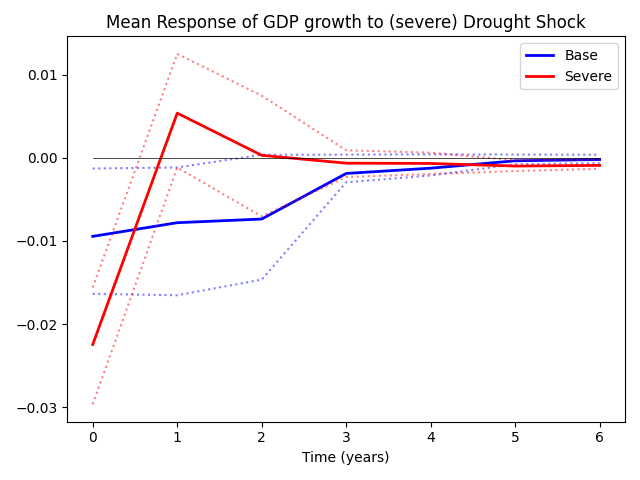
\includegraphics[width=\textwidth]{figures/BSBC/Developing/severe/severe_BSBC_devgrow_drought.png} 
    \end{subfigure}
    \begin{subfigure}[b]{0.32\textwidth}
        \centering
        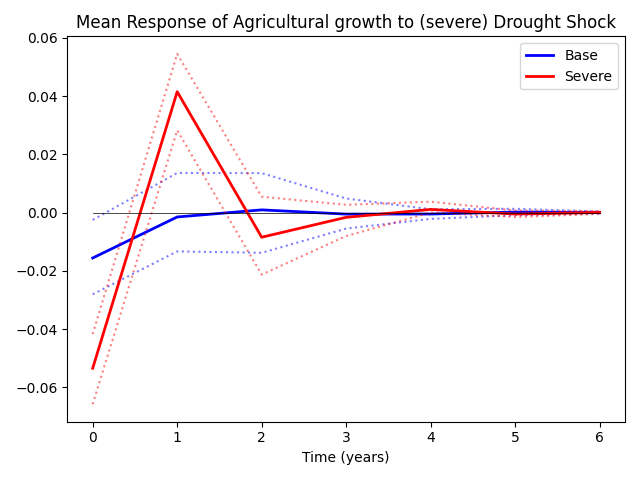
\includegraphics[width=\textwidth]{figures/BSBC/Developing/severe/severe_BSBC_devagr_drought.png}
    \end{subfigure}
    \begin{subfigure}[b]{0.32\textwidth}
        \centering
        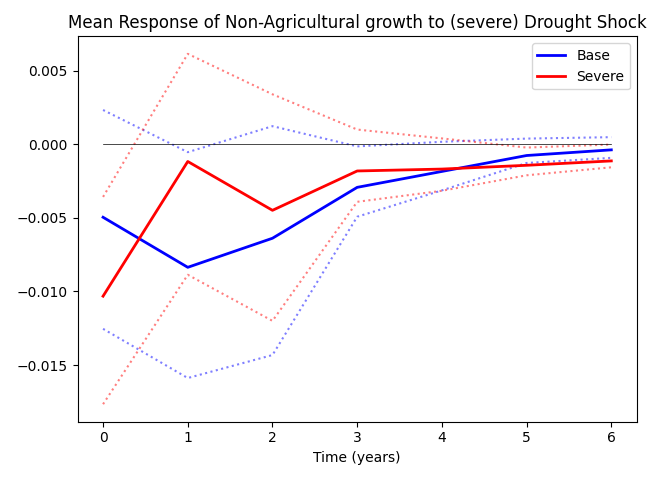
\includegraphics[width=\textwidth]{figures/BSBC/Developing/severe/severe_BSBC_devnon_drought.png}
    \end{subfigure}
    \caption*{Mean responses after adding severe natural disaster regressors to the model, where "severe" shows the sum of base effect and severe effect}
    \label{fig:guidance_scale}
\end{figure}
\end{frame}

\begin{frame}{Comparison with the Paper}

\begin{block}{Overall Assessment}
Our Python replication \textbf{successfully reproduces} the paper's findings. Coefficients match to the 4th decimal place, and significance levels are identical.
\end{block}

\vspace{0.3em}
\textbf{Key findings confirmed:}
\begin{itemize}
    \item \textcolor{myred}{Droughts} $\rightarrow$ consistently \textbf{negative} effect on GDP growth (strongest result)
    \item \textcolor{myblue}{Floods} $\rightarrow$ surprisingly \textbf{positive} effect, especially in Year 2 (recovery/reconstruction)
    \item Earthquakes $\rightarrow$ mixed effects, depends on severity and sector
    \item Storms $\rightarrow$ generally weak and insignificant effects
\end{itemize}

\vspace{0.3em}
\textbf{One discrepancy:}
\begin{itemize}
    \item Paper's Table III reports $N_{\text{obs}} = 2097$, but the author-provided dataset (\texttt{dev\_grow.xls}) contains 1866 rows. Similarly, provided samples for sectoral growth (agricultural/non-agricultural) are smaller than the paper reports. 
\end{itemize}
\end{frame}

\section{Experience \& Difficulties}

\begin{frame}{Difficulty \#1: Computational Cost}
\begin{alertblock}{The Problem}
The nested bootstrap (1000 $\times$ 1000 iterations of heavy matrix algebra) made the BSBC script \textbf{practically impossible} to run in pure NumPy, in which estimated runtime exceeded \textbf{10 hours}.
\end{alertblock}

\vspace{0.3em}
\textbf{Solution}: We used \texttt{numba} (JIT compilation) to accelerate the bottleneck functions:
\begin{itemize}
    \item \texttt{btst()} $\rightarrow$ the main bootstrap loop with recursive data generation
    \item \texttt{meanpsi()} $\rightarrow$ averaging impulse responses over $B\ (=1000)$ replications
    \item \texttt{psimat()} $\rightarrow$ computing the lag polynomial $\Psi(L) = \Phi(L)^{-1}\Theta(L)$
\end{itemize}

\vspace{0.3em}
\textbf{Result}: Runtime reduced from $\sim$10+ hours to $\sim$\textbf{25 minutes} ($\approx 25\times$ speedup), while preserving numerical equivalence with the pure Python version.
\end{frame}

\begin{frame}{Difficulty \#2: MATLAB $\rightarrow$ Python Translation}
\begin{columns}
\begin{column}{0.48\textwidth}
\textbf{Indexing differences:}
\begin{itemize}
    \item MATLAB is \textbf{1-indexed}, Python is \textbf{0-indexed}
    \item Every column reference (e.g., \texttt{vars(:,145)} $\rightarrow$ \texttt{vars[:,144]}) had to be carefully adjusted
    \item Array reshaping: MATLAB uses column-major (Fortran) order by default
\end{itemize}
\end{column}
\begin{column}{0.48\textwidth}
\textbf{Other challenges:}
\begin{itemize}
    \item Numba doesn't support all NumPy operations (had to restructure matrix code)
    \item Singular matrix errors when running the severe model on developed-country data (no severe floods recorded)
    \item Non-contiguous array slicing caused Numba performance warnings
\end{itemize}
\end{column}
\end{columns}
\end{frame}

\begin{frame}{Lessons Learned}
\begin{enumerate}
    \item \textbf{Replication is harder than it looks}: Even with complete code and data, translating between languages introduces subtle bugs. Having the original MATLAB code to compare against was essential.
    
    \vspace{0.3em}
    \item \textbf{Performance matters}: Computationally intensive methods like the nested bootstrap require thoughtful optimization. The original MATLAB code benefits from built-in compiled linear algebra; Python needed Numba to match.
    
    \vspace{0.3em}
    \item \textbf{Bootstrap is powerful but expensive}: The BSBC method elegantly corrects the Nickell bias without complex analytical derivations, but the nested bootstrap for inference turns a theoretically simple idea into a computationally heavy operation.
    
    \vspace{0.3em}
    \item \textbf{Results are robust}: The consistency between LSDV and BSBC estimates confirms that the economic response (especially for droughts and floods) is strong and not an artifact of the estimation method.
\end{enumerate}
\end{frame}

\section{Conclusion}

\begin{frame}{Summary}
\begin{columns}
\begin{column}{0.55\textwidth}
\textbf{The paper's main findings:}
\begin{itemize}
    \item Droughts are \textbf{unambiguously harmful}
    \item Floods can be \textbf{net positive} (reconstruction effect)
    \item Earthquakes show \textbf{mixed} effects depending on severity and sector
    \item Storms have \textbf{weak/insignificant} effects
    \item Severe disasters (mostly) amplify the impacts
\end{itemize}
\end{column}
\begin{column}{0.42\textwidth}
\textbf{Replication outcome:}
\begin{itemize}
    \item[\checkmark] All results \textbf{successfully replicated}
    \item[\checkmark] MATLAB $\rightarrow$ Python translation \textbf{validated}
    \item[\checkmark] Performance \textbf{optimized} with Numba JIT
    \item[\checkmark] Extended with formatted output tables
\end{itemize}
\end{column}
\end{columns}

\vspace{1em}
\begin{center}
\Large Thank you! \\ \normalsize Questions?
\end{center}
\end{frame}

\end{document}
